\section{Experiment}
	\begin{figure}[htbp]
	\centering
	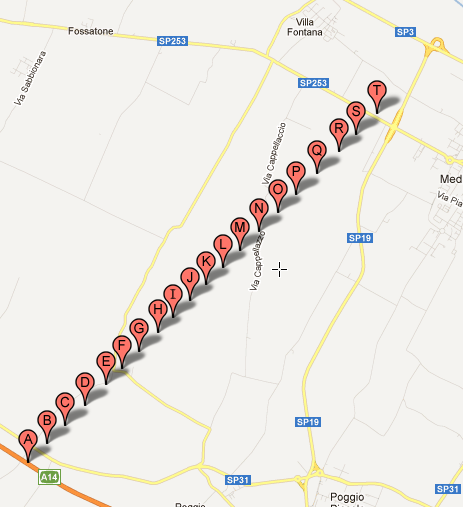
\includegraphics[trim = 0mm 0mm 0mm 10mm ,width=3.2in]{imgs/punti_mappa.png}
	\caption{Fake positions used for the experiment}
	\label{fig:positions_experiment}
	\end{figure}

To try out our testbed applications, we implemented the Fast Broadcast algorithm both for the Android and Desktop application. Simulations were made on a set of fake positions distributed on a straight line, each at a random distance between $275$ and $325$ meters from the preceding one, covering approximately $8$ kilometers. A graphical representation can be seen in figure \ref{fig:positions_experiment}.

\subsubsection{Android application}
To test our Android application we used three Android devices. 10 executions of the Fast Broadcast algorithm were performed, all with the following parameters:

\begin{center}
\begin{tabular}{|m{0.22\textwidth}|m{0.12\textwidth}|}
	\hline	
	\ttt{SLOT SIZE} 			& 250 ms \\
	\hline
	\ttt{CW MIN}				& 5\\
	\hline
	\ttt{CW MAX}				& 10\\
	\hline
	\ttt{ACTUAL RANGE}			& 1000 m\\
	\hline
	\ttt{DEFAULT RANGE}			& 300 m\\
	\hline
	\ttt{HELLO MESSAGE TURN}	& 500 ms\\
	\hline
\end{tabular}
\end{center}

%We first tried an execution wothout range estimation, then with range estimation phase. In the second case, the average amount of time waitd on the contention window by each device resulted to be smaller, and so the contention window size. However, due to the overhead introduced by Hello message exchanging and processing, a solution with static range performs a much faster message propagation.
%In both cases, the overhead introduced by TCP traffic doesn't let the algorithm beahave properly, resulting in some cases in simultaneous message forwarding by different devices.
Slot size was choosen to be $250ms$ to be great enought to reduce simultaneous retransmission of different devices; in fact we noticed that, due to TCP overhead, sometimes message transmission was too slow, resulting two devices forwarding the same message; Unfortunately this is unavoidable using Java and high level protocols, however this does not increase directly the number of hops, because redundant alert received are simply discarded.
During the application testing we tried to use UDP protocol to provide a much faster message transmission, but unfortunately the PER was too high to obtain a complete simulation: in some cases alert messages were lost, so the simulation ended before reaching the last position. We decided to use UDP protocol to exchange \textit{Hello} messages to relieve the TCP server from the traffic they generate.

% UDP EXPERIMENT
%The transport protocol we choose to send out Alert messages was UDP, this to reduce the protocol stack overhead (with TCP was estimated to be $\geq250$ms), speeding up the execution and let us set more realistic parameters values. This was achieved adding a filter to the transport manager at application startup. Hello messages were exchanged using TCP protocol, to reduce the traffic the UDP server thread had to manage.
Execution results are shown in table \ref{tab:Android_res}. Execution time, waited slots on contention window and contention window size are the average of the values measured in each device. As can be seen, the time needed to forward the Alert message to the last position is quite big; this is mainly due to slot size and TCP overhead. The number of Hops in some executions equals to the theoretical optimum (with this settings and three devices, optimal hop number is 15: our Fast Broadcast implementation simplistically assumes that when a device forwards a message, only (the two) following devices could hear it; more complex scenarious can be modeled).

\begin{table}
% increase table row spacing, adjust to taste
%\renewcommand{\arraystretch}{1}
% if using array.sty, it might be a good idea to tweak the value of
%\extrarowheight as needed to properly center the text within the cells
\caption{Fast Broadcast simulation results on Android, with Three devices}
\label{tab:Android_res}
\centering
% Some packages, such as MDW tools, offer better commands for making tables
% than the plain LaTeX2e tabular which is used here.
\begin{tabular}{|m{0.06\textwidth}|m{0.08\textwidth}|m{0.08\textwidth}|m{0.08\textwidth}|m{0.07\textwidth}|}
\hline
Execution & Total \newline Time (sec) & Average waited slots & Average Contention Window size & Hops \newline number \\
\hline
%1 & 17,0187 	& 626,667 	& 5,67 & 19 \\ % 2.506668
1 & 17,0187		& 2.506668 	& 5,67 & 19 \\
\hline
%2 & 15,1167 	& 581	  	& 5,33 & 15 \\ % 
2 & 15,1167 	& 2.324	  	& 5,33 & 15 \\ % 
\hline
% 3 & 22,0833	& 585,333 	& 5,33 & 15 \\ 
3 & 22,0833 	& 2.341332 	& 5,33 & 15 \\  
\hline
% 4 & 16,2190 	& 573	  	& 5,33 & 19 \\ % 2.292
4 & 16,2190 	& 2.292	  	& 5,33 & 19 \\ % 
\hline
% 5 & 23,3897 	& 644,333 & 6	 & 20 \\ % 2.577332
5 & 23,3897		& 2.5773 & 	6	 & 20 \\ % 2.5773
\hline
%6 & 22,2300 	& 639,667 	& 5	 & 18 \\ % 2.5587
6 & 22,2300 	& 2.5587 	& 5	 & 18 \\ % 
\hline
% 7 & 15,5160 	& 518	  	& 5,33 & 20 \\ % 2.072
7 & 15,5160 	& 2,072	  	& 5,33 & 20 \\ % 2.072
\hline
% 8 & 15,5780 	& 747,333 	& 6	 & 16 \\ % 2.989332
8 & 15,5780 	& 2.9893 	& 6	 & 16 \\ % 2.989332
\hline
% 9 & 15,6140 	& 606     	& 6	 & 15 \\ % 2.424
9 & 15,6140 	& 2.424     & 6	 & 15 \\ % 2.424
\hline
%10 & 18,997 	& 745,667 	& 5,67 & 17 \\ % 2.982668
10 & 18,997 	& 2.9827 	& 5,67 & 17 \\ % 2.982668
\hline
\end{tabular}
\end{table}  

\subsubsection{Desktop Application}

Execution results are shown in table \ref{tab:Desktop_res}. As can be seen, execution time is much smaller than the one required by the Android application. Data exchange via Raw Sockets reduces the transmission overhead dramatically, allowing for a smaller slot size and a more realistic simulation. However, we decided to use the same settings as for the Android simulation to allow direct confrontation of the results.

\begin{table}
% increase table row spacing, adjust to taste
%\renewcommand{\arraystretch}{1}
% if using array.sty, it might be a good idea to tweak the value of
%\extrarowheight as needed to properly center the text within the cells
\caption{Fast Broadcast simulation results with Desktop Application, with Three devices}
\label{tab:Desktop_res}
\centering
% Some packages, such as MDW tools, offer better commands for making tables
% than the plain LaTeX2e tabular which is used here.
\begin{tabular}{|m{0.06\textwidth}|m{0.08\textwidth}|m{0.08\textwidth}|m{0.08\textwidth}|m{0.07\textwidth}|}
\hline
Execution & Total \newline Time (sec) & Average waited slots & Average Contention Window size & Hops \newline number \\
\hline
1 & 9.143	& 3.5429	& 5.9143 	& 17 \\
\hline
2 & 8.78	& 2.8392  	& 5.53 		& 16 \\
\hline
3 & 10.695 	& 2.8049	& 5.5778 	& 18 \\
\hline
4 & 7.353 	& 2.5317  	& 5.467 	& 15 \\ 
\hline
5 & 8.456	& 2.6319 	& 5.578		& 15 \\
\hline
6 & 9.196	& 2.7024 	& 5.467		& 16 \\ 
\hline
7 & 7.169	& 2.1035	& 5.767		& 15 \\
\hline
8 & 8.978	& 2.4854	& 5.657		& 18 \\
\hline
9 & 8.743	& 2.7769	& 5.542		& 17 \\
\hline
10 & 7.286	& 2.6985 	& 5.34 		& 16 \\
\hline
\end{tabular}
\end{table}  
